\documentclass[12pt,a4paper,boxed,titlepage]{caspset}

% set 1-inch margins in the document
%\usepackage[left=1in,right=1in,top=1.2in,bottom=1in]{geometry}
\usepackage[left=1in,right=1in,top=1.2in,bottom=1in]{geometry}
\usepackage{lastpage}
% include this if you want to import graphics files with /includegraphics
\usepackage{graphicx}
\usepackage{hyperref}
\usepackage{amsmath,amsfonts,amsthm,amssymb}
\usepackage{setspace}
\usepackage{fancyhdr}
\usepackage{lastpage}
\usepackage{extramarks}
\usepackage{chngpage}
\usepackage{soul}
\usepackage[usenames,dvipsnames]{color}
\usepackage{graphicx,float,wrapfig}
\usepackage{ifthen}
\usepackage{listings}
\usepackage{courier}
\usepackage{multimedia}
\usepackage[toc,page,title,titletoc,header]{appendix}
\usepackage{multicol} 
\usepackage{xeCJK}
\usepackage{soul}
\usepackage{xcolor}



%\usepackage{fontspec}
\setCJKmainfont[BoldFont=simhei.ttf]{simsun.ttf}
%\setCJKsansfont{simhei.ttf}
%\setCJKmonofont{simfang.ttf}

%\setCJKmainfont{Adobe Song Std}
%\setCJKmainfont[BoldFont=Adobe Heiti Std]{Adobe Song Std}
%%%%%%%%%%%%%%%%%%%%%%%%%%%%%%%%%%%%%%%%%%%%%%%%%%%%%%

\graphicspath{{figures/}}

\setulcolor{red}

\setlength{\marginparwidth}{1in}

\newcommand{\hmwkTitle}{算法设计与分析}
\newcommand{\hmwkSubTitle}{第一章{~}复杂性分析初步} % No subtitle, so this will be excluded
\newcommand{\hmwkDueDate}{\today}
\newcommand{\hmwkClass}{信息工程学院}
\newcommand{\hmwkClassTime}{Tue/Thu{~}8:00}
\newcommand{\hmwkClassInstructor}{陈玉福}
\newcommand{\hmwkAuthorName}{周吕文}

%% Setup the header and footer
\pagestyle{fancy}                                                       %
\lhead{\hmwkAuthorName}                                                 %
\chead{\hmwkClass\ (\hmwkClassInstructor): \hmwkTitle}  %
\rhead{第\ \thepage\ 页, 共\ \protect\pageref{LastPage} 页}          %

\newcommand\invisiblesection[1]{%
  \refstepcounter{section}%
  \addcontentsline{toc}{section}{\protect\numberline{\thesection}#1}%
  \sectionmark{#1}}

\newcommand\invisiblesubsection[1]{%
  \refstepcounter{subsection}%
  \addcontentsline{toc}{subsection}{\protect\numberline{\thesubsection}#1}%
  \subsectionmark{#1}}


\makeatletter
\newcommand{\rmnum}[1]{\romannumeral #1}
\newcommand{\Rmnum}[1]{\expandafter\@slowromancap\romannumeral #1@}
\makeatother

\renewcommand\refname{\bf\large 参考文献}
\renewcommand\contentsname{\bf 目 \ \ \ 录}
\renewcommand\figurename{\bf 图}
\renewcommand\tablename{\bf 表}
\renewcommand{\appendixtocname}{附录}
\renewcommand{\appendixpagename}{附录}
\renewcommand\listfigurename{图目录}

\usepackage{listings} % 添加宏包
\definecolor{DarkGreen}{rgb}{0.0,0.3,0.0}
 \lstset %定义程序代码显示版面,可自定义 .
{language=c++,
numbers=left,
numberstyle=\ttfamily\scriptsize,
frame=single,
basicstyle=\ttfamily\small,
keywordstyle=\ttfamily\bf\color{Blue},
ndkeywordstyle=\ttfamily\bf\color{Brown},
commentstyle=\color{DarkGreen},
identifierstyle=\ttfamily\color{black}\bfseries,
stringstyle=\color{pink}\ttfamily,showstringspaces=false,
breaklines=true,
escapeinside=``
}

\begin{document}
\title{算法设计与分析(2011-2012秋)\\作业整理\\ \vspace{-20pt} }

\author{{\Large 授课老师:陈玉福}\\ \vspace{50pt}\\ 周吕文\\ \href{mailto:zhou.lv.wen@gmail.com}{zhou.lv.wen@gmail.com}\\ \vspace{50pt}}
\date{中国科学院力学研究所\\2011年11月28日}
%\tableofcontents
\maketitle 

\tableofcontents
\newpage

%\includepdf[pages=1-]{cover}
%\setcounter{page}{1}
\invisiblesection{第一章{~}复杂性分析初步}
\problemlist{\bf 第一章{~}复杂性分析初步}
\invisiblesubsection{习题1.1}
\begin{problem}[习题1.1]
试确定下述程序的执行步数,该函数实现一个$m\times n$矩阵与一个$n\times p$矩阵之间的乘法:

\centering
矩阵乘法运算
\begin{lstlisting}[language=C++][caption={c++}]
template<class T>
void Mult(T **a, T **b, int m, int n, int p)
{
  for(int i=0; i<m; i++)
    for(int j=0; j<p; j++){
      T sum=0;
      for(int k=0; k<n; k++)
        Sum+=a[i][k]*b[k][j];
      C[i][j]=sum;
    }
}
\end{lstlisting}
\end{problem}

\begin{solution}
\textbf{解:}表\ref{stepcount}是题中程序各行的执行步数统计.因此该程序执行的总步数为$\textrm{total step} = (m+1) +m(p+1)+mp+mp(n+1)+mpn +mp = 2mpn + 4mp+2m + 1$
\begin{table}[!htb]
\centering
\caption{\label{stepcount}矩阵乘法运算执行步数统计}
\begin{tabular}{|l|l|l|l|l|l|l|l|l|}
\cline{1-4}\cline{6-9}
\multicolumn{1}{|c|}{行数} & \multicolumn{1}{c|}{s/e} & \multicolumn{1}{c|}{频率} & \multicolumn{1}{c|}{总步数} & \multicolumn{1}{c|}{} & \multicolumn{1}{c|}{行数} & \multicolumn{1}{c|}{s/e} & \multicolumn{1}{c|}{频率} & \multicolumn{1}{c|}{总步数} \\
\cline{1-4}\cline{6-9}
\multicolumn{1}{|c|}{01} & \multicolumn{1}{c|}{0} & \multicolumn{1}{c|}{0} & \multicolumn{1}{c|}{0} & \multicolumn{1}{c|}{} & \multicolumn{1}{c|}{07} & \multicolumn{1}{c|}{1} & \multicolumn{1}{c|}{$mp(n+1)$} & \multicolumn{1}{c|}{$mp(n+1)$} \\
\multicolumn{1}{|c|}{02} & \multicolumn{1}{c|}{0} & \multicolumn{1}{c|}{0} & \multicolumn{1}{c|}{0} & \multicolumn{1}{c|}{} & \multicolumn{1}{c|}{08} & \multicolumn{1}{c|}{1} & \multicolumn{1}{c|}{$mpn$} & \multicolumn{1}{c|}{$mpn$} \\
\multicolumn{1}{|c|}{03} & \multicolumn{1}{c|}{0} & \multicolumn{1}{c|}{0} & \multicolumn{1}{c|}{0} & \multicolumn{1}{c|}{} & \multicolumn{1}{c|}{09} & \multicolumn{1}{c|}{0} & \multicolumn{1}{c|}{$mp$} & \multicolumn{1}{c|}{$mp$} \\
\multicolumn{1}{|c|}{04} & \multicolumn{1}{c|}{1} & \multicolumn{1}{c|}{$m+1$} & \multicolumn{1}{c|}{$m+1$} & \multicolumn{1}{c|}{} & \multicolumn{1}{c|}{10} & \multicolumn{1}{c|}{0} & \multicolumn{1}{c|}{0} & \multicolumn{1}{c|}{0} \\
\multicolumn{1}{|c|}{05} & \multicolumn{1}{c|}{1} & \multicolumn{1}{c|}{$m(p+1)$} & \multicolumn{1}{c|}{$m(p+1)$} & \multicolumn{1}{c|}{} & \multicolumn{1}{c|}{11} & \multicolumn{1}{c|}{0} & \multicolumn{1}{c|}{0} & \multicolumn{1}{c|}{0} \\
\multicolumn{1}{|c|}{06} & \multicolumn{1}{c|}{1} & \multicolumn{1}{c|}{$mp$} & \multicolumn{1}{c|}{$mp$} & \multicolumn{1}{c|}{} & \multicolumn{1}{c|}{} & \multicolumn{1}{c|}{} & \multicolumn{1}{c|}{} & \multicolumn{1}{c|}{} \\
\cline{1-4}\cline{6-9}
\end{tabular}
\end{table}
\end{solution}

\invisiblesubsection{习题1.5}
\begin{problem}[习题1.5]
下面那些规则是正确的?为什么?
\begin{enumerate}
\item $\big\{f(n)=O\big(F(n)\big), g(n)=O\big(G(n)\big)\big\}\Rightarrow f(n)/g(n)=O\big(F(n)/G(n)\big)$;
\item $\big\{f(n)=O\big(F(n)\big), g(n)=O\big(G(n)\big)\big\}\Rightarrow f(n)/g(n)=\Omega\big(F(n)/G(n)\big)$;
\item $\big\{f(n)=O\big(F(n)\big), g(n)=O\big(G(n)\big)\big\}\Rightarrow f(n)/g(n)=\Theta\big(F(n)/G(n)\big)$;
\item $\big\{f(n)=\Omega\big(F(n)\big), g(n)=\Omega\big(G(n)\big)\big\}\Rightarrow f(n)/g(n)=\Omega\big(F(n)/G(n)\big)$;
\item $\big\{f(n)=\Omega\big(F(n)\big), g(n)=\Omega\big(G(n)\big)\big\}\Rightarrow f(n)/g(n)=O\big(F(n)/G(n)\big)$;
\item $\big\{f(n)=\Theta\big(F(n)\big), g(n)=\Theta\big(G(n)\big)\big\}\Rightarrow f(n)/g(n)=\Theta\big(F(n)/G(n)\big)$;
\end{enumerate}
\end{problem}

\begin{solution}
\textbf{解:}对以题中6个小命题,错误的给出反例,正确的给出证明,具体如下:

\begin{enumerate}
\item \textbf{错误:} 在满足题设条件下,不妨设$f(n) = F(n) = g(n) = 1$, $G(n) = n$,
则显然不存在正常数$c$,当n足够大时使得:$1 = f(n)/g(n)\leq c F(n)/G(n) = c/n$.

\item \textbf{错误:} 在满足题设条件下,不妨设$f(n) = G(n) = g(n) = 1$, $F(n) = n$,
则显然不存在正常数$c$,当n足够大时使得:$1 = f(n)/g(n)\geq c F(n)/G(n) = cn$.

\item \textbf{错误:} 由1,2两小题中的反例,可知在满足题设条件下, $f(n)/g(n)$和$F(n)/G(n)$不一定同阶.

\item \textbf{错误:} 在满足题设条件下,不妨设$f(n) = F(n) = G(n) = 1$, $g(n) = n$,
则显然不存在正常数$c$,当n足够大时使得:$1/n = f(n)/g(n)\geq c F(n)/G(n) = c$.

\item \textbf{错误:} 在满足题设条件下,不妨设$F(n) = G(n) = g(n) = 1$, $f(n) = n$,
则显然不存在正常数$c$,当n足够大时使得:$ n = f(n)/g(n)\leq c F(n)/G(n) = c$.

\item \textbf{正确:} 由题意知:存在正常数$a_1$和$a_2$, 及$b_1$和$b_2$使得
\[
a_1F(n)\leq f(n) \leq a_2F(n), {~} b_1G(n)\leq g(n) \leq b_2G(n)
\]
则有
\[
\frac{a_1F(n)}{b_2G(n)}\leq \frac{f(n)}{g(n)} \leq \frac{a_2F(n)}{b_1G(n)}
\]
令$c_1 = a_1/b_2$, $c_2 = a_2/b_1$则有
\[
c_1\frac{F(n)}{G(n)}\leq \frac{f(n)}{g(n)} \leq c_2\frac{F(n)}{G(n)}
\]
\end{enumerate}
\end{solution}

\invisiblesubsection{习题1.6}
\begin{problem}[习题1.6]

\[
4n^2,{~} \log n,{~} 3^n,{~} 20n,{~} n^{2/3},{~} n!
\]
\end{problem}
\begin{solution}
\textbf{解:} 按照渐近阶从低到高的顺序排列上述表达式:
\[
\log n < n^{2/3} < 20n  < 4n^2 < 3^n < n!
\]
\end{solution}


\begin{problem}[习题1.7]
\begin{enumerate}
\item 假设某算法在输入规模是时为$T(n)=3*2^n$. 在某台计算机上实现并完成该算法的时间是$t$秒. 现有另一台计算机, 其运行速度为第一台的64倍, 那么, 在这台计算机上用同一算法在$t$秒内能解决规模为多大的问题?
\item 若上述算法改进后的新算法的计算为$T(n)=n^2$, 则在新机器上用$t$秒时间能解决输入规模为多大的问题?
\item 若进一步改进算法, 最新的算法的时间复杂度为$T(n)=8$, 其余条件不变, 在新机器上运行, 在$t$秒内能够解决输入规模为多大的问题?
\end{enumerate}
\end{problem}
\begin{solution}
\textbf{解:}
\begin{enumerate}
\item 设该算法在原计算机和新计算机上每步运行所需的时间分别为$t_1$, $t_2$, 则根据题意得:
\[
t_1 = \frac{t}{T(n)}, t_2 = \frac{t_1}{64}
\]
设该算法在新计算机上能解决的规模为$n'$,则有
\[
3\times 2^{n'}\times t_2 = 3\times 2^{n'}\times \frac{t_1}{64} = 3\times 2^{n}\times t_1
\]
解得$n'=n+6$, 因此在新计算机上用同一算法在$t$秒内能解决规模为$n+6$.

\item 算法改进后的新算法的计算为$T(n)=n^2$. 则有
\[
t = n'^2\times t_1 = 3\times 2^{n}\times t_1
\]
解得$n'=\sqrt{3\cdot 2^{n+6}}$. 因此在新计算机上$t$秒内能解决规模为$\sqrt{3\cdot 2^{n+6}}$.

\item 最新的算法的时间复杂度为$T(n)=8$. 则有
\[
t = 8\times t_1 = 3\times 2^n\times t_1
\]
显然上式与$n'$无关,即$T(n)$不随$n$变化,所以任意规模的$n'$都能在$t$秒内解决.

\end{enumerate}
\end{solution}

\invisiblesubsection{习题1.8}
\begin{problem}[习题1.8]
Fibonacci数有递推关系:
\begin{displaymath}
F(n)\left\{ \begin{array}{ll}
1, & n = 0 \\
1, & n = 1 \\
F(n-1) + F(n-2), & n>1
\end{array} \right.
\end{displaymath}
试求出$F(n)$的表达.
\end{problem}
\begin{solution}
\textbf{解:}设当$n>3$时$F(n)$, $F(n-1)$, $F(n-2)$满足:
\[
F(n)=F(n-1) + F(n-2)
\]
故其特征方程为
\[
\lambda ^2 = \lambda + 1
\]
解得:$\lambda_1 = (1+\sqrt{5})/2$, $\lambda_2=(1-\sqrt{5})/2$, 则可设
\[
F(n) = a \lambda_1^n + b\lambda_2^n
\]
由$F(2)=2$, $F(3)=3$, 解得$a=\frac{1+\sqrt{5}}{2\sqrt{5}}$, $b = -\frac{1-\sqrt{5}}{2\sqrt{5}}$
因此有
\[
F(n) = \frac{1}{\sqrt{5}} = \Big[\big(\frac{1+\sqrt{5}}{2}\big)^{n+1}- \big(\frac{1-\sqrt{5}}{2}\big)^{n+1}\Big]
\]

%化简并与已知条件比较:
%\[
%F(n) = (\beta - \alpha) F(n-1) + \beta\alpha F(n-2) \Longleftrightarrow F(n) = F(n-1) + F(n-2)
%\]
%得$\beta - \alpha = 1$, $\alpha\beta = 1$. 不妨设$\alpha>0, \beta>0$, 可解得$\alpha = (\sqrt{5}-1)/2$, $\beta = (\sqrt{5}+1)/2$. 所以$\{F(n)+\alpha F(n-1)\}$为等比数列, 公比为$\beta$. 因此有
%{\setlength\arraycolsep{2pt}
%\begin{eqnarray}
%F(n)+\alpha F(n-1) & = & (F(1)+\alpha F(0))\beta^{n-1}
%\nonumber\\
%& = & (1+\alpha)\beta^{n-1}
%\nonumber\\
%& = & \beta^{n}\nonumber
%\end{eqnarray}}
%因此有
%\begin{eqnarray}
%F(n) & = & \alpha F(n-1) + \beta^{n}
%\nonumber\\
%& = & \alpha (\alpha F(n-2) + \beta^{n-1}) +  \beta^{n}
%\nonumber\\
%& = & \alpha^2 F(n-2) + \alpha\beta^{n-1} +  \beta^{n}
%\nonumber\\
%& = & \alpha^{n-1} F(1) + \alpha^n+ \alpha^{n-1}\beta+ \cdots + \alpha\beta^{n-1} +  \beta^{n}
%\nonumber\\
%\end{eqnarray}}

\end{solution}


\newpage
\invisiblesection{第二章{~}图与遍历算法}
\problemlist{\bf 第二章{~}图与遍历算法}
\invisiblesubsection{习题2.1}
\begin{problem}[习题2.1]
证明下列结论:
\begin{enumerate}
\item 在一个无向图中, 如果每个顶点的度大于等于2, 则该该图一定含有圈;
\item 在一个有向图D中, 如果每个顶点的出度都大于等于1, 则该图一定含有一个有向圈.
\end{enumerate}
\end{problem}
\begin{solution}
\begin{enumerate}
\item \textbf{证:} 设该无向图无圈,有$m$条边,$n$个顶点. 则该无向图为树或森林,因此满足$m=n-k$,又由如果每个顶点的度大于等于2有
\[
\sum d(v) = 2|E| = 2m \geq 2n
\]
故有
\begin{equation}\label{q1}
m \geq n \Longrightarrow n - k \geq n, (k = 1,2,\cdots)
\end{equation}
显然式(\ref{q1})是不成立的,故假设该无向图无圈成立,即该该图一定含有圈.
\item \textbf{证:} 设该有向图中的最长有向迹为$P=V_1V_2\cdots V_k$,
又因为每个顶点的度大于等于1, 故存在$V'$为$V_k$连接到的点,若$V' \notin P$, 则$V_1V_2\cdots V_kV'$比$P$更长,与假设矛盾. 因此, $V'\in P$, 设$V'=V_n(n\leq k)$, 故存在有向圈$V_nV_{n+1}\cdots V_kV_n$
\end{enumerate}
\end{solution}

\invisiblesubsection{习题2.5}
\begin{problem}[习题1.5]
实现图的D-搜索算法. 要求用ALGEN语言写出算法的伪代码, 或者用一种计算机高级语言写出程序.
\end{problem}
\begin{solution}
\textbf{解:}先将起始顶点存入栈中. 搜索时, 取出栈顶元素, 遍历其邻点, 将未搜索的存入栈, 遍历其邻点后, 重复此过程, 直至栈变为空栈.
\begin{table}[!htb]
\centering
\caption{\label{DsearchG}图的D-搜索算法伪代码}
\begin{tabular}{llllll}
\hline
\multicolumn{6}{l}{\textbf{Proc  DBFT(G,m)}\textcolor{blue}{ //m为不连通分支数}} \\
 & \multicolumn{5}{l}{ count:=0 ;\textcolor{blue}{//计数器,标示已经被访问的顶点个数}} \\
 & \multicolumn{5}{l}{\textbf{for} i \textbf{to} n \textbf{do}} \\
 &  & \multicolumn{4}{c}{visited[i]:=0;\textcolor{blue}{ //数组visited标示各顶点被访问的序数,其元素初始化为0.}} \\
 & \multicolumn{5}{l}{\textbf{end{for}}} \\
 & \multicolumn{5}{l}{\textbf{for} i to m \textbf{do}  \textcolor{blue}{//遍历不连通分支的情况}} \\
 &  & \multicolumn{4}{l}{\textbf{ if} visited[i]=0 then} \\
 &  &  & \multicolumn{3}{l}{DBFS (i); } \\
 &  & \multicolumn{4}{l}{\textbf{end\{if\}}} \\
 & \multicolumn{5}{l}{\textbf{end\{for\}}} \\
\multicolumn{6}{l}{\textbf{end\{DBFT\}}} \\
\hline
\end{tabular}
\end{table}
表\ref{DsearchG}是图的D-搜索算法伪代码. 表\ref{DsearchG}中调用的DBFS为由一点出发的D-搜索,其伪代码见表\ref{DsearchV}
\newpage
\begin{table}[!htb]
\centering
\caption{\label{DsearchV}由一点出发的D-搜索算法伪代码}
\begin{tabular}{llllll}
\hline
\multicolumn{6}{l}{\textbf{Proc DBFS(v)} } \\
\multicolumn{6}{l}{\textcolor{blue}{//数组visited标示各顶点被访问的序数,其元素初始化为0}} \\
\multicolumn{6}{l}{\textcolor{blue}{// 计数器count计数到目前为止已经被访问的顶点个数, 初始化为0}} \\
 & \multicolumn{5}{c}{ PushStack (v , S); \textcolor{blue}{//首先访问v,将S初始化为只含有一个元素v的栈}} \\
 & \multicolumn{5}{l}{count :=count +1; visited[v] := count;} \\
 & \multicolumn{5}{l}{\textbf{While}  S 非空 \textbf{do}} \\
 &  & \multicolumn{4}{l}{u :=PullHead(S); \textcolor{blue}{//取出栈顶的元素u, 并从栈中删除}} \\
 &  & \multicolumn{4}{l}{\textbf{for} 邻接于u的所有顶点w  \textbf{do}} \\
 &  &  & \multicolumn{3}{l}{\textbf{if}  visited[w] = 0 \textbf{then}} \\
 &  &  &  & \multicolumn{2}{l}{PushStack(w,S); \textcolor{blue}{//将w存入栈S}} \\
 &  &  &  & \multicolumn{2}{l}{ count :=count +1; visited[w] := count;} \\
 &  &  & \multicolumn{3}{l}{\textbf{end\{if\}}} \\
 &  & \multicolumn{4}{l}{\textbf{end\{for\}}} \\
 & \multicolumn{5}{l}{\textbf{end\{while\}}} \\
\multicolumn{6}{l}{\textbf{end\{DBFS\}}} \\
\hline
\end{tabular}
\end{table}
\end{solution}

\invisiblesubsection{习题2.6}
\begin{problem}[习题2.6]右图的无向图以邻接链表存储,
\vspace{-2em}
\begin{multicols}{2}
~

而且在关于每个顶点的链表中与该顶点相邻的顶点是按照字母顺序排列的.
试以此图为例描述讲义中算法DFNL的执行过程.

\begin{center}
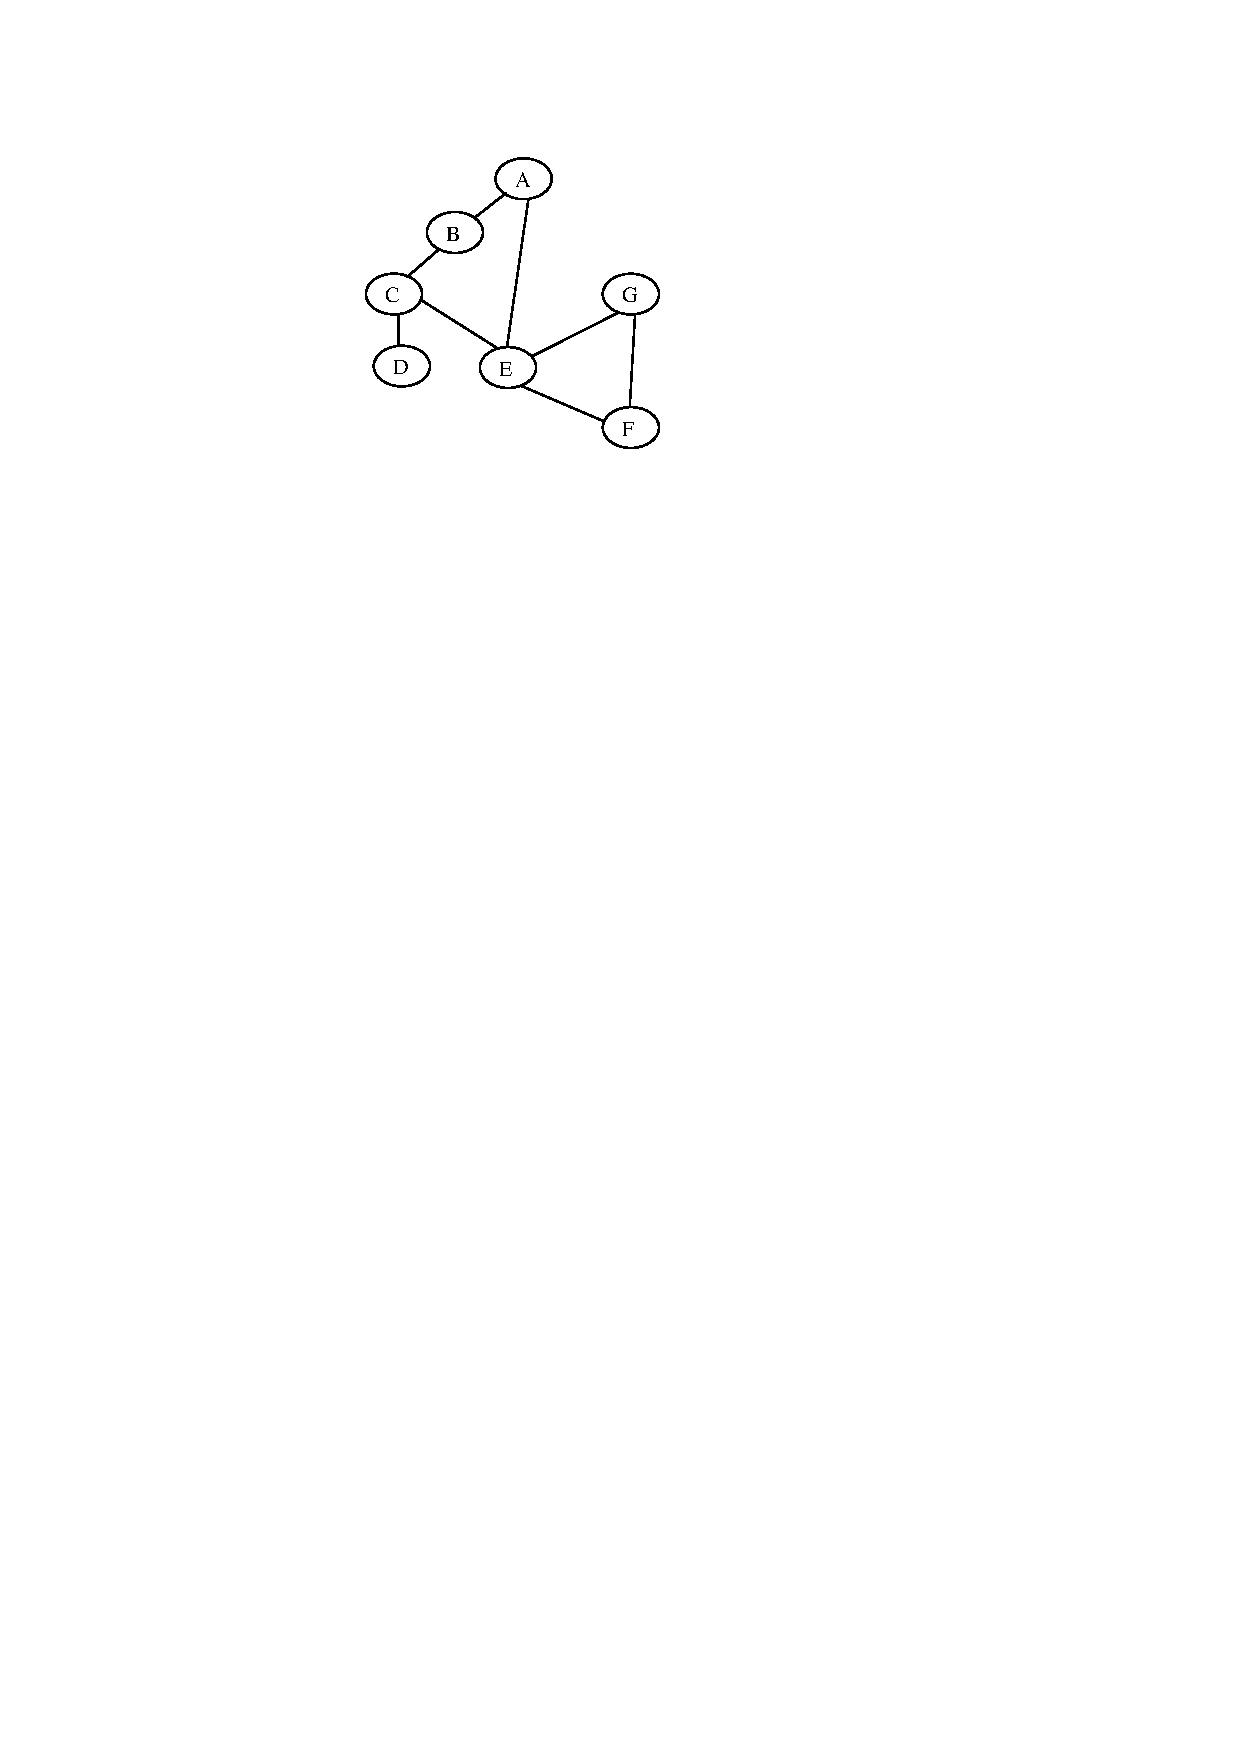
\includegraphics[width=0.12\textwidth]{fig01.pdf}\\
一个无向图$G$
\end{center}

\end{multicols}

\end{problem}
\begin{solution}
\textbf{解:}题中所给的无向图所对应的邻接链表如图\ref{link}所示.
\begin{figure}[!htb]
\centering
\begin{tabular}{l|l|l|l|l|l|l|l|llllll}
\cline{2-2}\cline{4-5}\cline{7-8}
A & { ~ } & $\rightarrow$ & B &  & $\rightarrow$ & E & 0 &  &  &  &  &  &  \\
\cline{2-2}\cline{4-5}\cline{7-8}
B &  & $\rightarrow$ & A &  & $\rightarrow$ & C & 0 &  &  &  &  &  &  \\
\cline{2-2}\cline{4-5}\cline{7-8}\cline{10-11}
C &  & $\rightarrow$ & B &  & $\rightarrow$ & D &  & \multicolumn{1}{l|}{$\rightarrow$} & \multicolumn{1}{l|}{E} & \multicolumn{1}{l|}{0} &  &  &  \\
\cline{2-2}\cline{4-5}\cline{7-8}\cline{10-11}
D &  & $\rightarrow$ & C & 0 & \multicolumn{1}{l}{} & \multicolumn{1}{l}{} & \multicolumn{1}{l}{} &  &  &  &  &  &  \\
\cline{2-2}\cline{4-5}\cline{7-8}\cline{10-11}\cline{13-14}
E &  & $\rightarrow$ & A &  & $\rightarrow$ & C &  & \multicolumn{1}{l|}{$\rightarrow$} & \multicolumn{1}{l|}{F} & \multicolumn{1}{l|}{} & \multicolumn{1}{l|}{$\rightarrow$} & \multicolumn{1}{l|}{G} & \multicolumn{1}{l|}{0} \\
\cline{2-2}\cline{4-5}\cline{7-8}\cline{10-11}\cline{13-14}
F &  & $\rightarrow$ & E &  & $\rightarrow$ & G & 0 &  &  &  &  &  &  \\
\cline{2-2}\cline{4-5}\cline{7-8}
G &  & $\rightarrow$ & E &  & $\rightarrow$ & F & 0 &  &  &  &  &  &  \\
\cline{2-2}\cline{4-5}\cline{7-8}
\end{tabular}
\caption{\label{link}无向图的邻接链表}
\end{figure}
此图讲义中算法DFNL的执行过程如下:\\
{\small
\begin{tabular}{lllllll}
\multicolumn{7}{l}{初始化  数组DFN:=0,  num=1;} \\
 & \multicolumn{6}{l}{A为树的根节点,对A计算DFNL(A,null), DFN(A):=num=1; L(A):=num=1; num:=1+1=2.} \\
 & \multicolumn{6}{l}{从邻接链表查到A的邻接点B,} \\
 &  & \multicolumn{5}{l}{因为DFN(B)=0,对B计算DFNL(B,A), DFN(B):= num=2; L(B):=num=2; num:=2+1=3.} \\
 &  & \multicolumn{5}{l}{查邻接链表得到B的邻接点A, 因为DFN(A)=1 0, 但A=A, 即是B的父节点,无操作.} \\
 &  & \multicolumn{5}{l}{接着查找邻接链表得到B的邻接点C,因为DFN(C)=0,} \\
 &  &  & \multicolumn{4}{l}{对C计算DFNL(C,B), DFN(C):= num=3;  L(C):=num=3; num:=3+1=4.} \\
 &  &  & \multicolumn{4}{l}{查找C的邻接点B,因为DFN(B)=1≠0, 但B=B,即是C的父节点, 无操作.} \\
 &  &  & \multicolumn{4}{l}{接着查找邻接链表得到C的邻接点D,因为DFN(D)=0,} \\
 &  &  &  & \multicolumn{3}{l}{对D计算 DFNL(D,C), DFN(D):= num=4;   L(D):=num=4;  num:=4+1=5.} \\
 &  &  &  & \multicolumn{3}{l}{查找得D邻接点C,而DFN(C)=3≠0,但C=C,为D的父节点, L(D)保持不变.} \\
 &  &  &  & \multicolumn{3}{l}{D的邻接链表结束,DFNL(D,C)的计算结束.} \\
 &  &  & \multicolumn{4}{l}{返回到D的父节点C,查找邻接链表得到C的邻接点E, 因为DFN(E)=0,} \\
 &  &  &  & \multicolumn{3}{l}{对E计算DFNL(E,C), DFN(E):=num=5;   L(E):=num=5;   num:5+1=6;} \\
 &  &  &  & \multicolumn{3}{l}{查找得E邻接点A,因DFN(A)=1≠0,又A≠C,变换L(E)=min(L(E), DFN(A))=1.} \\
 &  &  &  & \multicolumn{3}{l}{查找得E邻接点C,因DFN(C)=3≠0,但C=C,无操作.} \\
 &  &  &  & \multicolumn{3}{l}{查找得E邻接点F, 因DFN(F)=0,} \\
 &  &  &  &  & \multicolumn{2}{l}{对F计算 DFNL(F,E), DFN(F):=num=6;   L(F):=num=6;  num:=6+1=7;} \\
 &  &  &  &  & \multicolumn{2}{l}{查找得F邻接点E,因DFN(E)=5≠0,但E=E,无操作.} \\
 &  &  &  &  & \multicolumn{2}{l}{查找得F邻接点G,因DFN(G)=0,} \\
 &  &  &  &  &  & 对G计算 DFNL(G,F),DFN(G):=num=7;   L(G):=num=7;  num=7+1=8; \\
 &  &  &  &  &  & 查找G邻接点E,因DFN(E)=5≠0,又E≠F,L(G)=min(L(G),DFN(E))=5 \\
 &  &  &  &  &  & 查找得G邻接点F,因DFN(F)=6≠0,但F=F,无操作. \\
 &  &  &  &  &  &  G的邻接链表结束,DFNL(G,F)的计算结束. \\
 &  &  &  &  &  & L(F):=min(L(F),L(G))=min(6,5)=5 \\
 &  &  &  &  & \multicolumn{2}{l}{F的邻接链表结束,DFNL(F,E)的计算结束.} \\
 &  &  &  &  & \multicolumn{2}{l}{L(E):=min(L(E),L(F))=min(1,5)=1} \\
 &  &  &  & \multicolumn{3}{l}{E邻接链表结束, DFNL(E,C)计算结束.} \\
 &  &  &  & \multicolumn{3}{l}{L(C):=min(L(C),L(E))=min(3,1)=1} \\
 &  &  & \multicolumn{4}{l}{C的邻接链表结束,DFNL(C,B)计算结束.} \\
 &  &  & \multicolumn{4}{l}{L(B):=min(L(B),L(C))=min(2,1)=1} \\
 &  & \multicolumn{5}{l}{查找B的邻接链表结束,DFNL(B,A)计算结束.} \\
 &  & \multicolumn{5}{l}{L(A):=min(L(A),L(B))=1} \\
 & \multicolumn{6}{l}{查找得A的邻接点E,因DFN(E)=0,又E≠null,则L(A)=min(L(A),DFN(E))=1} \\
\multicolumn{7}{l}{查找A的邻接链表结束,DFNL(A,null)计算结束.} \\
\end{tabular}
}

\end{solution}

\invisiblesubsection{习题2.7}
%%%%%%%%%%%%%%%%%%%%%%%%%%%%%%%%%%%%%%%%%%%%%%%%%%%%%%%%%%%%%%%%%%%%%%%%%%%%%%%%%%%%%%%%%%%%%%%%%%%%%%%%%
\begin{problem}[习题2.7]
对图的另一种检索方法是D-Search. 该方法与BFS的不同之处在于将队列换成栈, 即下一个要检测的结点是最新加到未检测结点表的那个结点.
\begin{enumerate}
\item 写一个D-Search算法;
\item 证明由结点v开始的D-Search能够访问$v$可到达的所有结点;
\item 你的算法的时, 空复杂度是什么?
\end{enumerate}
\end{problem}

\begin{solution}
\begin{enumerate}
\item \textbf{解:} D-Search算法如习题1.5中的表\ref{DsearchV}所示.
\item \textbf{证:} 设$v_n$为$v$可到达的某一节点, $v$与$v_n$间的迹为$P = vv_1v_2\cdots v_n$. 由表\ref{DsearchV}的算法可知, $v$最先被放入栈,并被访问. 其后取出栈顶元素并访问, 同时其邻接的顶点被放入栈中,重复此过程,直至栈变空. 因此当$v$被取出时$v_1$将被放出栈中, 其后当$v_1$被取出时,$v_1$被访问的同时, $v_1$的邻点$v_2$被放入栈中. 假设$v_k$与$v_{k+1}$相邻, 若$v_k$可访问,则$v_{k+1}$也可被访问.下面用数学规纳法证明题设:
    \begin{itemize}
    \item 显然该假设对于$v(v_0)$,$v_1$成立.
    \item 当$v_k$可访问时, $v_k$的所有邻点,包括$v_{k+1}$将被放入栈中, 栈中的顶点将逐个被取出访问, 因此$v_{k+1}$也将被访问.
    \end{itemize}
    所以, D-Search能够访问$v$可到达的结点$v_n$. 由于$v_n$是任意假设的, 因此D-Search能够访问$v$可到达的所有结点.
\item \textbf{解:} 图$G$的D-搜索算法能够访问$G$中由$v$可能到达的所有顶点
    如果记$t(v,\varepsilon)$ 和$s(v,\varepsilon)$ 为D-搜索算法在任意一个具有$v$个顶点和
    $\varepsilon$条边的连通图$G$上所花的最大时间和最大空间.则可证明其时空复杂度:
\begin{itemize}
\item 除节点$v$外, 只有当结点$w$满足$visited[w]$才被存入栈中, 因此每个节点至多有一次被存入栈中, 需要的栈空间至多是$v-1$; $visited$数组需要的空间为$v$; 其于变量所用空间为$O(1)$, 所以该算法的空间复杂度为$s(v,\varepsilon) = \Theta(v)$.
\item 如果使用邻接链表, 语句for循环要做$d(u)$次, 而语句while循环需要做$v$次,
    因而整个循环做$\sum_{u\in V}d(u)=2\varepsilon$次$O(1)$操作, 又$visited$, 和$count$的赋值都需要$v$次操作, 因此时间复杂度为$t(v,\varepsilon) = \Theta(v+\varepsilon)$
\item 如果采用邻接矩阵, 则语句while循环总共需要做$v^2$次操作, $visited$和$count$的赋值都需要$v$次操作, 因而时间复杂度为$t(v,\varepsilon) = \Theta(v^2)$.
\end{itemize}
\end{enumerate}
\end{solution}

\invisiblesubsection{习题2.8}

\begin{problem}[习题2.8]
考虑下面这棵假想的对策树:
\begin{center}
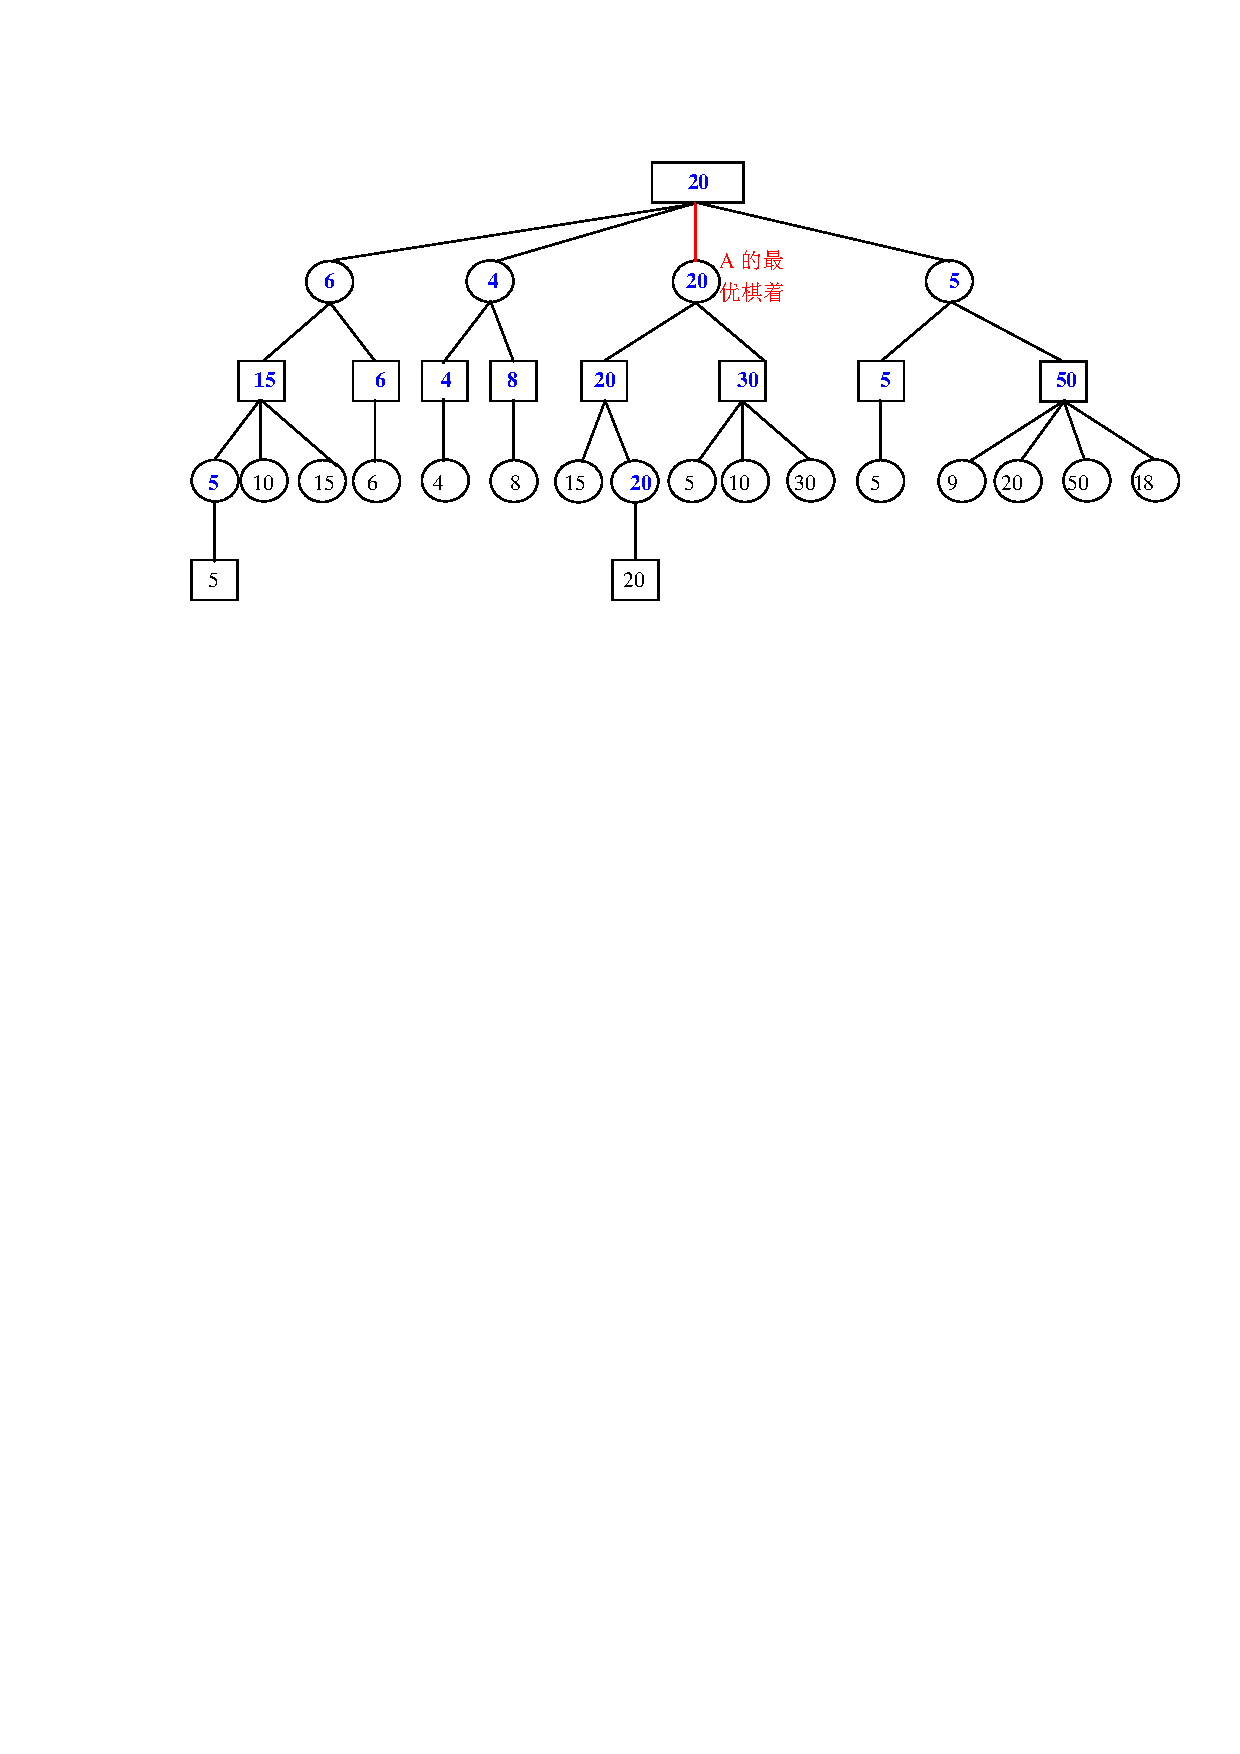
\includegraphics[width=0.8\textwidth]{fig02.pdf}\\
\end{center}
\begin{enumerate}
\item 使用最大最小方法(2-4-2)式获取各结点的值;
\item 弈者$A$为获胜应该什么棋着?
\item 列出算法$VEB$计算这棵对策树结点的值时各结点被计算的顺序;
\item 对树中每个结点$X$,用(2-4-3)式计算$V(X)$;
\item 在取$X=\textrm{根}$,$l=10$, $LB=-\infty$, $D=\infty$的情况下, 用算法$AB$计算此树的根的值期间, 这棵树的那些结点没有计算?
\end{enumerate}
\end{problem}
\begin{solution}
\begin{enumerate}
\item 各结点的值已在题中所给图中标出;
\item 弈者$A$为获胜应该走的棋着已在题中所给图中标出;
\item 算法$VEB$计算这棵对策树结点的值时各结点被计算的顺序如图\ref{ans34}中的红色数字;
\item 对树中每个结点$X$,用(2-4-3)式计算$V(X)$所得的值,已标在图\ref{ans34}中的方框或圆圈中(蓝色数字);
\begin{figure}[!htb]
\centering
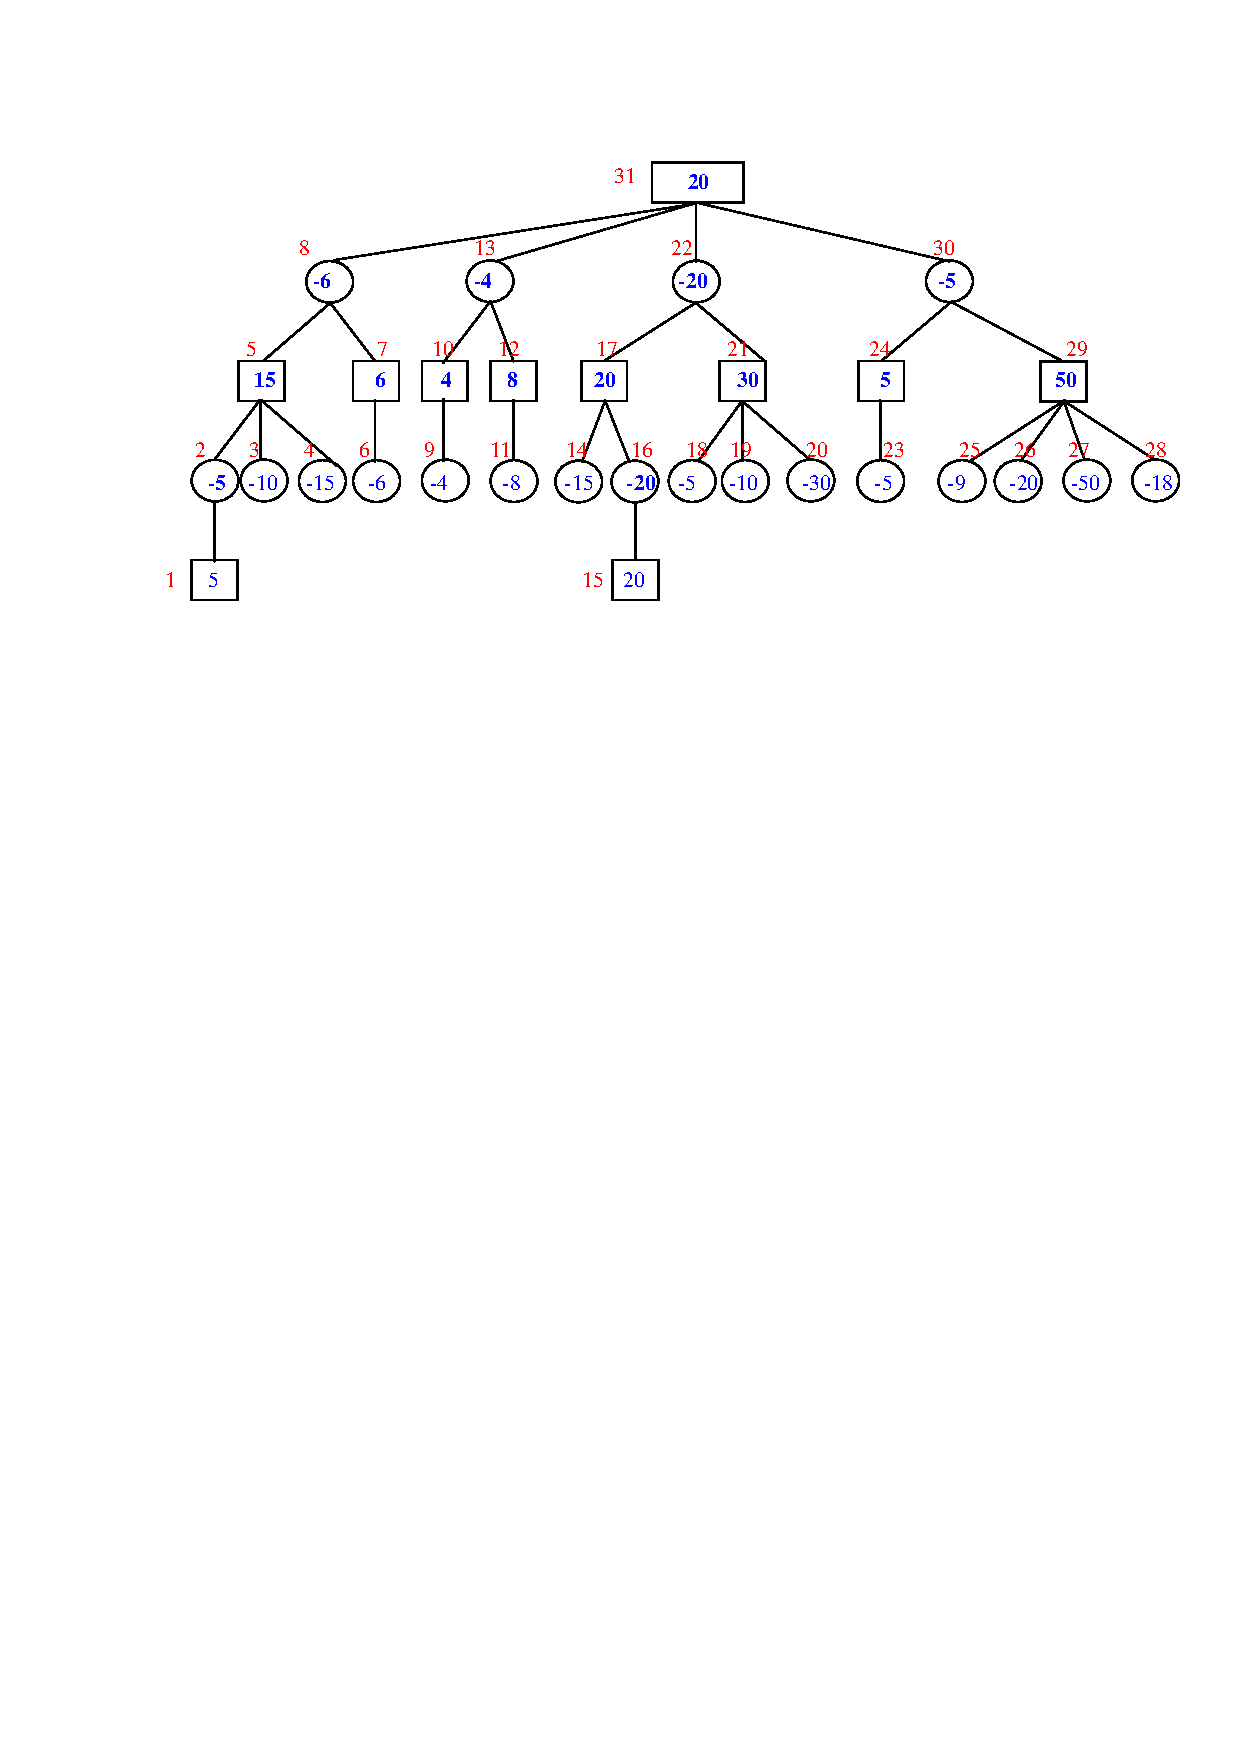
\includegraphics[width=0.8\textwidth]{fig02_1.pdf}
\caption{\label{ans34}第(3)(4)小问解}
\end{figure}
\item 在取$X=\textrm{根}$,$l=10$, $LB=-\infty$, $D=\infty$的情况下, 图\ref{ans34}中标有以下红色数字中的结点没有被计算:
    \[
    11, 12, 25, 26, 27, 28, 29
    \]
\end{enumerate}
\end{solution}


\newpage
\invisiblesection{第三章{~}分治算法}
\problemlist{\bf 第三章{~}分治算法}
\invisiblesubsection{习题3.1}
\begin{problem}[习题3.1]
编写程序实现归并排序算法MergeSortL和快速排序算法QuickSort;
\end{problem}
\begin{solution}
\textbf{解:}归并排序算法和快速排序算法的C++程序见附录\ref{sec:sort}(含时间复杂性测试).
\end{solution}

\invisiblesubsection{习题3.4}
\begin{problem}[习题3.4]
说明算法PartSelect的平均时间复杂性为$O(n)$.\\
\textbf{提示}:假定数组中的元素各不相同, 且第一次划分时划分元素$v$是第$i$小元素的概率为$1/n$. 因为Partition中的case语句所要求的时间都是$O(n)$, 所以, 存在常数$c$, 使得算法PartSelect 的平均时间复杂度$C_A^k(n)$可以表示为
\[
C_A^k(n)\leq cn+\frac{1}{n}\sum_{1\leq i < k}C_A^{k-1}(n-i) + \sum_{k<i\leq n}(C_A^k(i-1))
\]
令$R(n)=\max(C_A^k(n))$, 取$c\geq R(1)$试证明$R(n)\leq 4cn$
\end{problem}
\begin{solution}
\textbf{证:}设$C_A^k(n)$表示在含$n$个元素的数组$A$中搜索第$k$小元素的平均时间复杂度, 假定数组中的元素各不相同, 且第一次划分时划分元素$v$是第$i$小元素的概率为$1/n$. 因为Partition中的case语句所要求的时间都是$O(n)$, 所以, 存在常数$c$, 使得算法PartSelect 的平均时间复杂度$C_A^k(n)$可以表示为
\[
C_A^k(n)\leq cn+\frac{1}{n}\sum_{1\leq i < k}C_A^{k-1}(n-i) + \sum_{k<i\leq n}(C_A^k(i-1))
\]
令$R(n)=\max(C_A^k(n))$, 取$c\geq R(1)/4$. 当$n=2$时, 有
\[
R(2)\leq 2c + \frac{1}{2}R(1)=2c+2c = 4c
\]
设对于$n>2$的所有自然数,$R(n)\leq 4cn$, 则有
{\setlength\arraycolsep{2pt}
\begin{eqnarray}
R(n) & \leq & cn+\frac{1}{n}\Big(\sum_{1\leq i< k}R(n-i) + \sum_{k\leq i<n}R(i-1)\Big)
\nonumber\\
& \leq & cn + \frac{4c}{n}\Big(\sum_{1\leq i< k}(n-i) + \sum_{k\leq i<n}(i-1)\Big)
\nonumber\\
& \leq & cn + \frac{4c}{n}\Big(\frac{(k-1)(2n-k)}{2}+\frac{(n-k)(k+n-1)}{2}\Big)
\nonumber\\
& \leq & cn - \frac{4c}{n}\frac{(k-1)(2n-k)+(n-k)(k+n-1)}{2}
\nonumber\\
& \leq & cn - \frac{4c}{n}\Big(k^2-(n+1)k-\frac{n^2-3n}{2}\Big)
\nonumber\\
& \leq & cn - \frac{4c}{n}\Big(-(\frac{n+1}{2})^2-\frac{n^2-3n}{2}\Big)
\nonumber\\
& \leq & cn + c\frac{3n^2-4n+1}{n}
\nonumber\\
& \leq & cn + 3c(n-1)
\nonumber\\
& \leq & 4cn
\nonumber
\end{eqnarray}}
因此, 平均时间复杂度为$C_A^k(n)\leq 4cn$, 故有$C_A^k(n) = O(n)$.
\end{solution}


\newpage
\invisiblesection{第四章{~}贪心算法}
\problemlist{\bf 第四章{~}贪心算法}
\invisiblesubsection{习题4.1}
\begin{problem}[习题4.1]
设有$n$个顾客同时等待一项服务. 顾客$i$需要的服务时间为$t_i$, $1\leq i\leq n$. 应该如何安排$n$个顾客的服务次序才能使总的等待时间达到最小? 总的等待时间是各顾客等待服务的时间的总和. 试给出你的做法的理由(证明).
\end{problem}
\begin{solution}
\textbf{解:}所需服务时间越短的顾客, 排在越前面. 即有$t_1\leq t_2\leq \cdots \leq t_n$. 其中下标为服务的顺序. 下面证明其为最优解.\\
\textbf{证:}设$T=[t_1,t_2,\cdots,t_i,\cdots,t_n]$, $t_i\leq t_{i+1}$不是最优解. $Y=[y_1,y_2,\cdots,y_i,\cdots,y_n]$ 是最优解,则必存在$i$使得$y_i>y_{i+1}$
则对于解$Y$, 各顾客等待服务的时间总和为
{\setlength\arraycolsep{2pt}
\begin{eqnarray}
T_{Y} & = & \underbrace{0}_{1}+ \underbrace{y_1}_{2} + \underbrace{y_1+y_2}_{3} + \cdots + \underbrace{y_1+\cdots + y_{i}}_{i+1} + \cdots + \underbrace{y_1+\cdots + y_{n-1}}_{n}\nonumber\\
& = & (n-1)y_1 + (n-2)y_2 +\cdots +(n-i)y_i + (n-(i+1))y_{i+1} + \cdots + 2y_{n-2} + y_{n-1}\nonumber\\
& > & (n-1)y_1 + (n-2)y_2 +\cdots +(n-i)y_{i+1} + (n-(i+1))y_{i} + \cdots + 2y_{n-2} + y_{n-1}\nonumber
\end{eqnarray}}
因此, $Y'=[y_1,y_2,\cdots,y_{i+1},y_i\cdots,y_n]$比$Y$更优, 因此$Y$不是最优解, 故假设不成立. 因此$T=[t_1,t_2,\cdots,t_i,\cdots,t_n]$, $t_i\leq t_{i+1}$是最优解.

\end{solution}

\invisiblesubsection{习题4.2}
\begin{problem}[习题4.2]
字符a-h出现的频率分布恰好是前8个Fibonacci数, 它们的Huffman编码是什么? 将结果推广到$n$个字符的频率分布恰好是前$n$个Fibonacci数的情形. Fibonacci数的定义为: $F_0=1$, $F_1=1$, $F_n = F_{n-2}+F_{n-1}$ if $n>1$.
\end{problem}
\begin{solution}
\textbf{解:}根据Fibonacci数的定义求可求出的a-h出现的频率分布, 再由Huffman编码算法可得到Huffman编码树. Huffman编码算法执行过程如图\ref{ah}
\begin{figure}[!htb]
\begin{minipage}[b]{.4\textwidth}
\centering
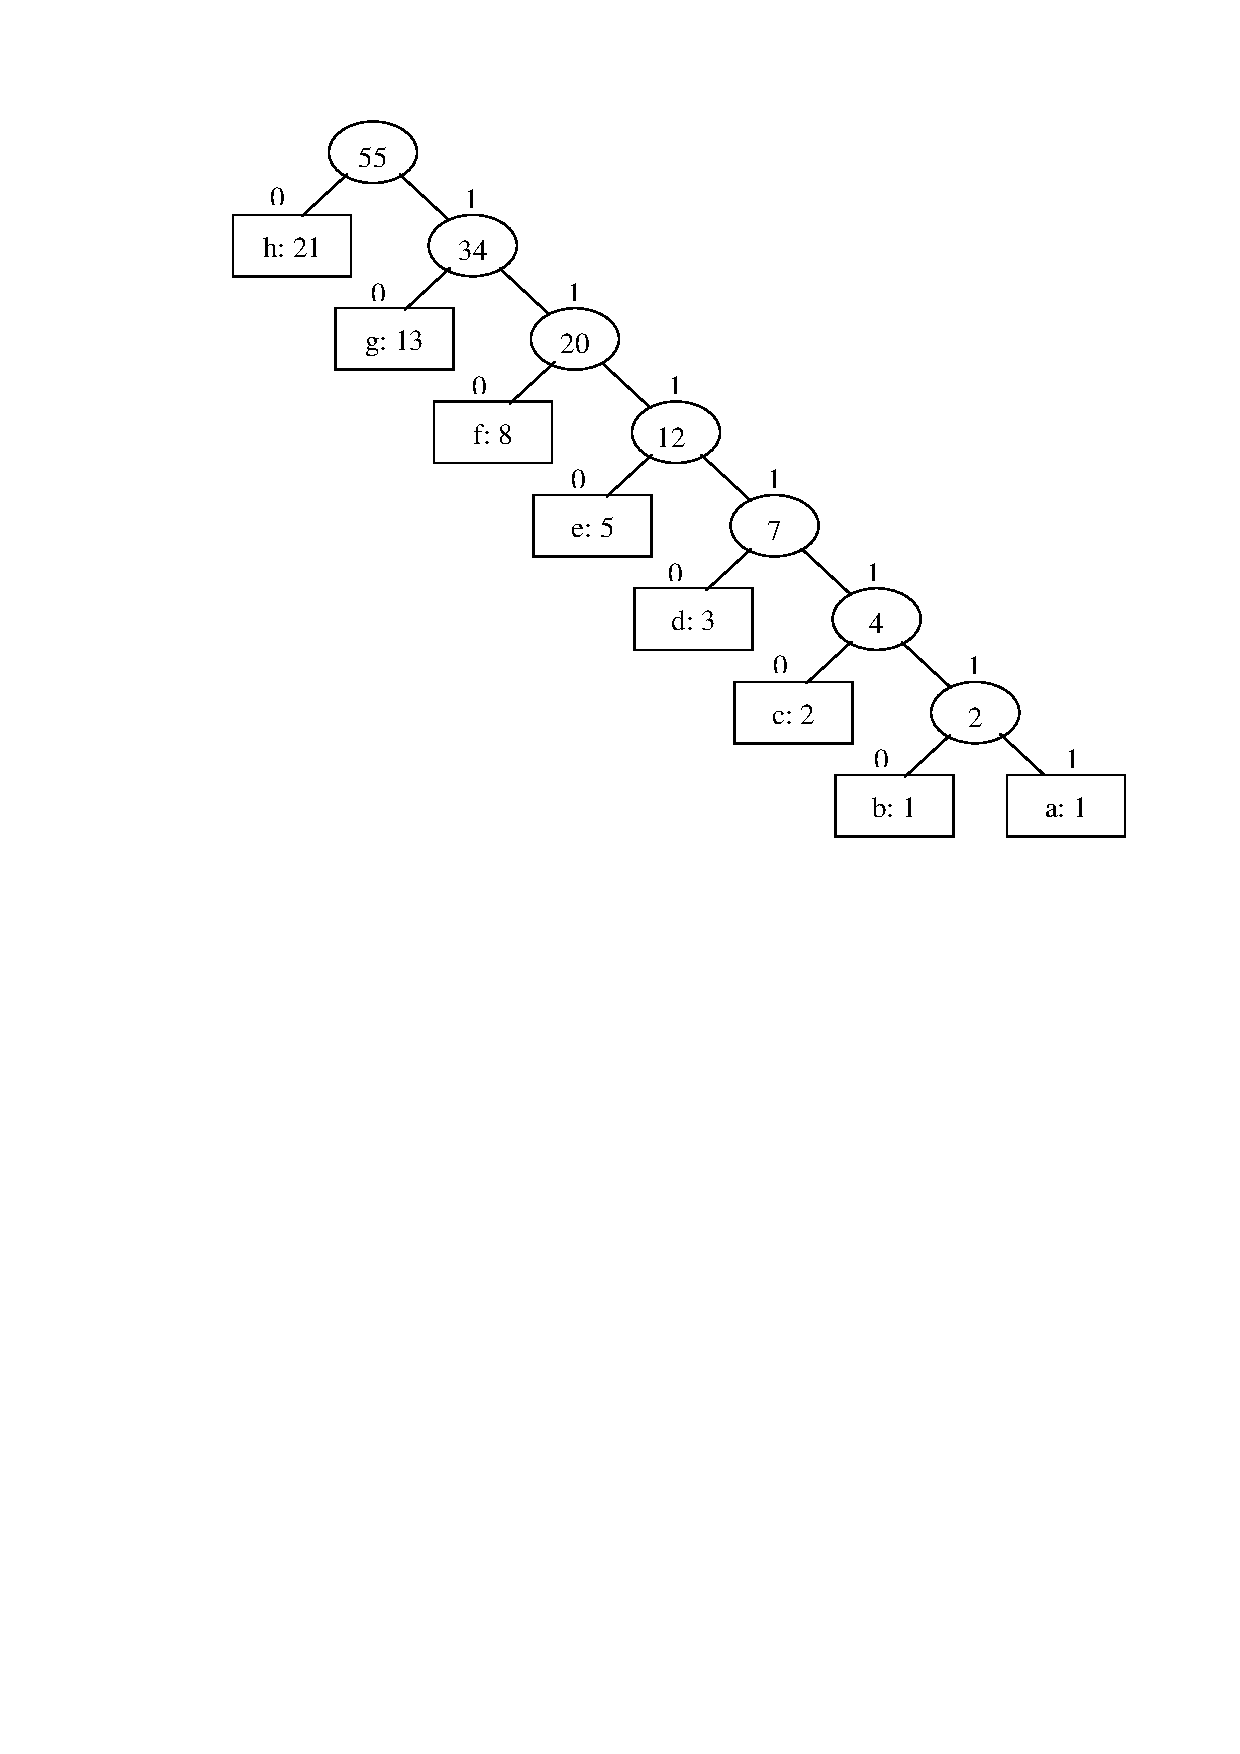
\includegraphics[width=0.8\textwidth]{tree.pdf}
\caption{\label{tree}Huffman编码树}
\end{minipage}%
\begin{minipage}[b]{.6\textwidth}
\centering
\begin{tabular}{l|llllll|l|l|}
\cline{2-9}
1 & \multicolumn{1}{l|}{a:1} & \multicolumn{1}{l|}{b:1} & \multicolumn{1}{l|}{c:2} & \multicolumn{1}{l|}{d:3} & \multicolumn{1}{l|}{e:5} & f:8 & g:13 & h:21 \\
\cline{2-9}
2 & \multicolumn{1}{l|}{c:2} & \multicolumn{2}{l|}{a+b:2} & \multicolumn{1}{l|}{d:3} & \multicolumn{1}{l|}{e:5} & f:8 & g:13 & h:21 \\
\cline{2-9}
3 & \multicolumn{1}{l|}{d:3} & \multicolumn{3}{l|}{(a+b)+c:4} & \multicolumn{1}{l|}{e:5} & f:8 & g:13 & h:21 \\
\cline{2-9}
4 & \multicolumn{1}{l|}{e:5} & \multicolumn{4}{l|}{( (a+b)+c )+d:7} & f:8 & g:13 & h:21 \\
\cline{2-9}
5 & \multicolumn{1}{l|}{f:8} & \multicolumn{5}{l|}{( ( (a+b)+c ) + d) +e:12} & g:13 & h:21 \\
\cline{2-9}
6 & \multicolumn{1}{l|}{g:13} & \multicolumn{6}{l|}{( ( ( (a+b)+c ) + d) +e ) + f:20} & h:21 \\
\cline{2-9}
7 & \multicolumn{1}{l|}{h:21} & \multicolumn{7}{l|}{( ( ( ( (a+b)+c ) + d) +e ) + f ) + g:34} \\
\cline{2-9}
8 & \multicolumn{8}{l|}{( ( ( ( ( (a+b)+c ) + d) +e ) + f ) + g ) + h:55} \\
\cline{2-9}
\end{tabular}
\caption{\label{ah}Huffman编码算法执行过程}
\end{minipage}
\end{figure}
因此, 可得到a-h的Huffman编码, 如图\ref{tree}所示. 可进一步将结果推广到$n$个字符的频率分布恰好是前$n$个Fibonacci数的情形, 第$i$个数的Huffman编码为
\begin{displaymath}
\left\{ \begin{array}{ll}
\overbrace{1\cdots 1}^{n-1\textrm{个}} & i = 1\\
\underbrace{1\cdots 1}_{n-i\textrm{个}}0 & 0< i \leq n\\
\end{array} \right.
\end{displaymath}
\end{solution}

\invisiblesubsection{习题4.3}
\begin{problem}[习题4.3]
设$p_1$, $p_2$, $\cdots$, $p_n$是准备存放到长为$L$的磁带上的$n$个程序, 程序$p_i$需要
的带长为$a_i$. 设$\sum_{i=1}^n>L$, 要求选取一个能放在带上的程序的最大子集合(即其中含有最多个数的程序)$Q$. 构造$Q$的一种贪心策略是按$a_i$的非降次序将程序计入集合.
\begin{enumerate}
\item 证明这一策略总能找到最大子集$Q$, 使得$\sum_{p_i\in Q}\leq L$.
\item 设$Q$是使用上述贪心算法得到的子集合, 磁带的利用率可以小到何种程度?
\item 试说明1问中提到的设计策略不一定得到使取最大值的子集合.
\end{enumerate}
\end{problem}

\begin{solution}
\begin{enumerate}
\item \textbf{证:}设$a_1\leq a_2\leq \cdots\leq a_n$是按非降次序排列的. 设贪心策略构造的最大子集$Q=[a_1, a_2, \cdots, a_m]$ 使得
    \[\sum_{i=1}^m a_i\leq L ,  \sum_{i=1}^{m+1} a_i> L\]

    假设$Q$不是最大子集, 则至少存在$m+1$个元素的集合$P=[a_{i_1}, a_{i_2}, \cdots, a_{i_{m+1}}]$ 使得
    \[\sum_{j=1}^{m+1} a_{i_j}\leq L ,  \sum_{j=1}^{m+2} a_{i_j}> L\]

    因为$a_1\leq a_2\leq \cdots\leq a_n$是按非降次序排列的, 所以有
    \[
    L<\sum_{i=1}^{m+1} a_i < \sum_{j=1}^{m+1} a_{i_j}
    \]
    这与假设是矛盾的, 因为不存大于$m$个元素的集合, 即这一策略总能找到最大子集$Q$, 使得$\sum_{p_i\in Q}\leq L$.
\item \textbf{解:}磁带的利用率为
\[
\alpha=\frac{\sum_{p_i\in Q}}{L}
\]
显然当$a_1>L$时$\alpha=0$, 因此磁带的利用率最小可为$0$.
\item \textbf{解:}贪心策略构总能找到最大子集$Q$, 只表示$Q$中的元素能达到最大$m$, 并不表示能使得放在带上的程序最长. 如果存在
    \[a_{m+1}+\sum_{i=1}^{m-1} a_i\leq L\]
    显然其利用率比贪心策略构出的$Q$大, 因此1问中提到的设计策略不一定得到使取最大值的子集合.
\end{enumerate}
\end{solution}

\newpage
\invisiblesubsection{习题4.4}
\begin{problem}[习题4.4]
写出Huffman编码的伪代码, 并编程实现.
\end{problem}
\begin{solution}
\textbf{解:}Huffman编码的伪代码见表\ref{huffmanArithmetic}. 其中函数Extract-Min(Q)是从Q中取出频率最小的节点.
\begin{table}[!htb]
\centering
\caption{\label{huffmanArithmetic}Huffman编码的伪代码}
\begin{tabular}{llll}
\hline
\multicolumn{4}{l}{\textbf{Proc} Huffman(A)\textcolor{blue}{//A为需要编码的字符集}} \\
 & \multicolumn{3}{l}{n = $|A|$;} \\
 & \multicolumn{3}{l}{Q = 按频率分布从小到大排序A} \\
 & \multicolumn{3}{l}{\textbf{for} i \textbf{to} n \textbf{do}} \\
 &  & \multicolumn{2}{l}{z = 新节点} \\
 &  & \multicolumn{2}{l}{left(z) = Extract-Min(Q); \textcolor{blue}{//取出Q中的第一个节点,并从Q中删去}} \\
 &  & \multicolumn{2}{l}{right(z) = Extract-Min(Q); \textcolor{blue}{//取出Q中的第一个节点,并从Q中删去}} \\
 &  & \multicolumn{2}{l}{frequency(z) =  frequency(left(z)) + frequency(right(z))} \\
 &  & \multicolumn{2}{l}{Insert(Q, z); \textcolor{blue}{//向Q中按频率顺序插入新节点}} \\
 & \multicolumn{3}{l}{\textbf{end\{for\}}} \\
 & \multicolumn{3}{l}{\textbf{return} Extract-Min(Q)} \\
\multicolumn{4}{l}{\textbf{end}\{Huffman\}} \\
\hline
\end{tabular}
\end{table}

实现的具体C++代码见附录\ref{sec:Huffman}. 在linux下经g++编译并运行得到图\ref{huffmanResult}.
\begin{figure}[!htb]
\centering
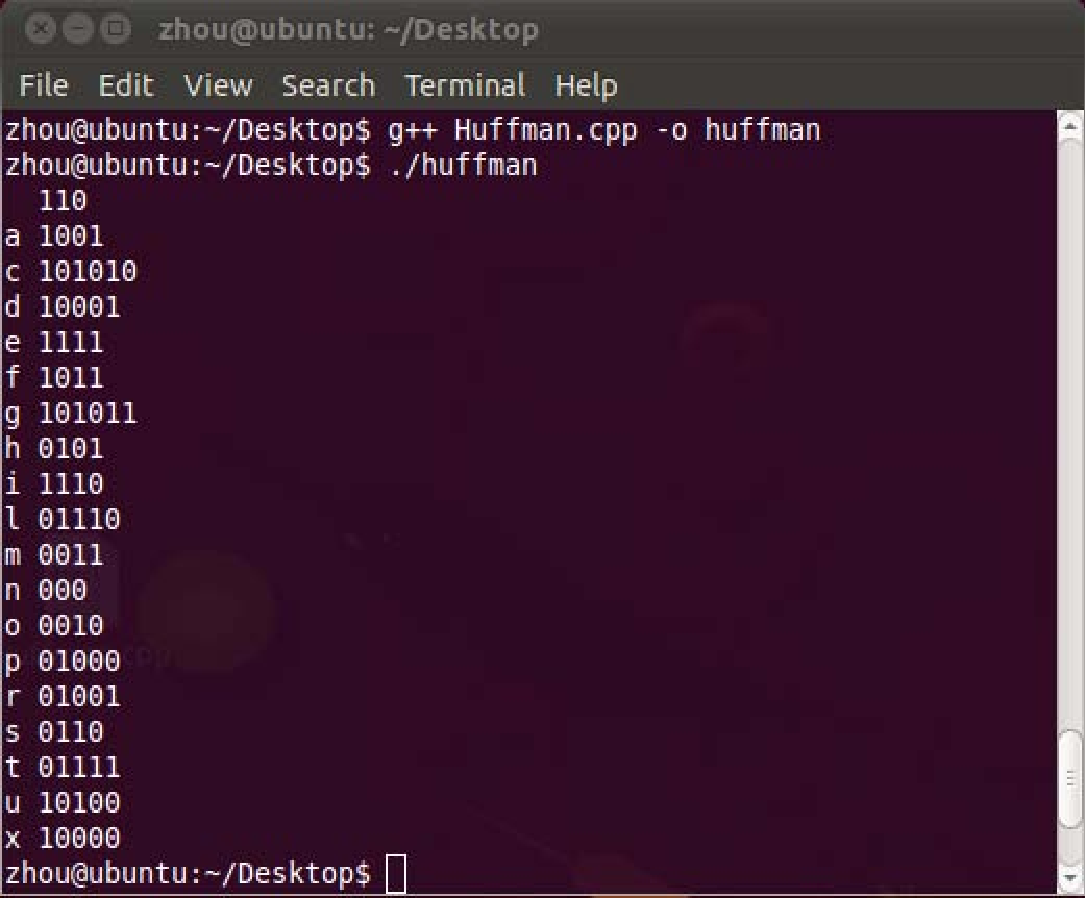
\includegraphics[width=0.7\textwidth]{huffman.pdf}
\caption{\label{huffmanResult}Huffman编码C++程序运行结果}
\end{figure}

\end{solution}


\newpage
\invisiblesection{第五章{~}动态规划算法}
\problemlist{\bf 第五章{~}动态规划算法}
\invisiblesubsection{习题5.1}
\begin{problem}[习题5.1]
最大子段和问题:给定整数序列$a_1, a_2, \cdots, a_n$, 求该序列形如$\sum_{k=i}^j a_k$的子段和的最大值:
$\max\{0, \max\limits_{1\leq i\leq j\leq n}\sum_{k=i}^j a_k\}$.
\begin{enumerate}
\item 已知一个简单算法如下:
\begin{lstlisting}[language=C++][caption={c++}]
int Maxsum(int n,int a,int& besti,int& bestj)
{ int sum = 0;
  for(int i=1;i<=n;i++){
     int suma = 0;
     for(int j=i;j<=n;j++){
        suma + = a[j];
        if(suma > sum){
          sum = suma;
          besti = i;
          bestj = j; }
     }
  }
  return sum;
}
\end{lstlisting}
试分析该算法的时间复杂性.
\item 试用分治算法解最大子段和问题, 并分析算法的时间复杂性.
\item 试说明最大子段和问题具有最优子结构性质, 并设计一个动态规划算法解最大子段和问题. 分析算法的时间复杂度.\\
(提示: 令$b(j) = \max\limits_{1\leq i\leq j\leq n}\sum_{k=i}^j a_k, j = 1, 2, \cdots, n$)
\end{enumerate}
\end{problem}
\begin{solution}
\begin{enumerate}
\item \textbf{解:}该简单算法的执行步数统见表\ref{stepnum}.
\begin{table}[!htb]
\centering
\caption{\label{stepnum}执行步数统计表}
\begin{tabular}{|l|l|l|l|l|l|l|l|l|}
\cline{1-4}\cline{6-9}
\multicolumn{1}{|c|}{行数} & \multicolumn{1}{c|}{s/e} & \multicolumn{1}{c|}{频率} & \multicolumn{1}{c|}{总步数} & \multicolumn{1}{c|}{} & \multicolumn{1}{c|}{行数} & \multicolumn{1}{c|}{s/e} & \multicolumn{1}{c|}{频率} & \multicolumn{1}{c|}{总步数} \\
\cline{1-4}\cline{6-9}
\multicolumn{1}{|c|}{01} & \multicolumn{1}{c|}{0} & \multicolumn{1}{c|}{0} & \multicolumn{1}{c|}{0} & \multicolumn{1}{c|}{} & \multicolumn{1}{c|}{08} & \multicolumn{1}{c|}{1} & \multicolumn{1}{c|}{n(n-1)/2} & \multicolumn{1}{c|}{n(n-1)/2} \\
\multicolumn{1}{|c|}{02} & \multicolumn{1}{c|}{0} & \multicolumn{1}{c|}{0} & \multicolumn{1}{c|}{0} & \multicolumn{1}{c|}{} & \multicolumn{1}{c|}{09} & \multicolumn{1}{c|}{1} & \multicolumn{1}{c|}{n(n-1)/2} & \multicolumn{1}{c|}{n(n-1)/2} \\
\multicolumn{1}{|c|}{03} & \multicolumn{1}{c|}{1} & \multicolumn{1}{c|}{n+1} & \multicolumn{1}{c|}{n+1} & \multicolumn{1}{c|}{} & \multicolumn{1}{c|}{10} & \multicolumn{1}{c|}{1} & \multicolumn{1}{c|}{n(n-1)/2} & \multicolumn{1}{c|}{n(n-1)/2} \\
\multicolumn{1}{|c|}{04} & \multicolumn{1}{c|}{1} & \multicolumn{1}{c|}{n+1} & \multicolumn{1}{c|}{n+1} & \multicolumn{1}{c|}{} & \multicolumn{1}{c|}{11} & \multicolumn{1}{c|}{0} & \multicolumn{1}{c|}{0} & \multicolumn{1}{c|}{0} \\
\multicolumn{1}{|c|}{05} & \multicolumn{1}{c|}{1} & \multicolumn{1}{c|}{n(n+1)/2} & \multicolumn{1}{c|}{n(n+1)/2} & \multicolumn{1}{c|}{} & \multicolumn{1}{c|}{12} & \multicolumn{1}{c|}{0} & \multicolumn{1}{c|}{0} & \multicolumn{1}{c|}{0} \\
\multicolumn{1}{|c|}{06} & \multicolumn{1}{c|}{1} & \multicolumn{1}{c|}{n(n-1)/2} & \multicolumn{1}{c|}{n(n-1)/2} & \multicolumn{1}{c|}{} & \multicolumn{1}{c|}{13} & \multicolumn{1}{c|}{0} & \multicolumn{1}{c|}{0} & \multicolumn{1}{c|}{0} \\
\multicolumn{1}{|c|}{07} & \multicolumn{1}{c|}{1} & \multicolumn{1}{c|}{n(n-1)/2} & \multicolumn{1}{c|}{n(n-1)/2} & \multicolumn{1}{c|}{} & \multicolumn{1}{c|}{14} & \multicolumn{1}{c|}{0} & \multicolumn{1}{c|}{0} & \multicolumn{1}{c|}{0} \\
\cline{1-4}\cline{6-9}
\end{tabular}
\end{table}
由表\ref{stepnum}可知该简单算法执行的总步数为:
$2\times (n+1)+n(n+1)/2 + 5\times n(n-1)/2 = 6n^2+4$
 所以该算法时间复杂度为$O(n^2)$.

\item 解最大子段的分治算法: 对给定序列$a[1:n]$对半划分为$a[1:\lfloor n/2\rfloor]$, $a[\lfloor n/2\rfloor+1:n]$, 并分别求出这两段的最大子段. 则原序列的最大子段有以下可能:
    \begin{itemize}
    \item 原序列的最大子段 = $a[1:\lfloor n/2\rfloor]$最大子段.
    \item 原序列的最大子段 = $a[\lfloor n/2\rfloor+1:n]$最大子段.
    \item 原序列的最大子段 = $a[1:\lfloor n/2\rfloor]$最大子段与$a[\lfloor n/2\rfloor+1:n]$最大子段组合.
    \end{itemize}
基于以上分析, 可得到解最大子段分治算法的伪代码, 见表\ref{MaxSubSum}.
\begin{table}[!htb]
\centering
\caption{\label{MaxSubSum}解最大子段分治算法的伪代码}
\begin{tabular}{lllll}
\hline
\multicolumn{5}{l}{\textbf{Proc} MaxSubSum(a, left, right)\textcolor{blue}{// a为整数序列}} \\
 & \multicolumn{4}{l}{\textbf{if} left $<$ right \textbf{then}} \\
 &  & \multicolumn{3}{l}{middle = $\lfloor\textrm{(left+right)}/2\rfloor$} \\
 &  & \multicolumn{3}{l}{MaxSumLeft = MaxSubSum(a, left, middle)} \\
 &  & \multicolumn{3}{l}{MaxSumRight = MaxSubSum(a,  middle+1, right)} \\
 &  & \multicolumn{3}{l}{sumleft =0; maxleft = 0;} \\
 &  & \multicolumn{3}{l}{\textbf{for} i \textbf{from} middle \textbf{to} left} \\
 &  &  & \multicolumn{2}{l}{sumleft = sumleft + a(i)} \\
 &  &  & \multicolumn{2}{l}{maxleft = \textbf{max}(sumleft, maxleft)} \\
 &  & \multicolumn{3}{l}{\textbf{end\{for\}}} \\
 &  & \multicolumn{3}{l}{sumright =0; maxright = 0;} \\
 &  & \multicolumn{3}{l}{\textbf{for} i \textbf{from} middle+1 \textbf{to} right} \\
 &  &  & \multicolumn{2}{l}{sumright = sumright + a(i)} \\
 &  &  & \multicolumn{2}{l}{maxright = \textbf{max}(sumright, maxright)} \\
 &  & \multicolumn{3}{l}{\textbf{end\{for\}}} \\
 &  & \multicolumn{3}{l}{SumCombine = maxleft+maxright}\\
 &  & \multicolumn{3}{l}{MaxLightRight = \textbf{max}(MaxSumLeft, MaxSumRight)} \\
 &  & \multicolumn{3}{l}{MaxSum = \textbf{max}(SumCombine, MaxLightRight)} \\
 &  & \multicolumn{3}{l}{\textbf{return} MaxSum} \\
 & \multicolumn{4}{l}{\textbf{else}} \\
 &  & \multicolumn{3}{l}{MaxSum = \textbf{max}(a(left),0)} \\
 &  & \multicolumn{3}{l}{\textbf{return} MaxSum} \\
\multicolumn{5}{l}{\textbf{end\{Proc\}}} \\
\hline
\end{tabular}
\end{table}\\
该算法的时间复杂度$T(n)$有递归关系式$T(n)=2T(n/2)+O(n), n>1$, $T(1) = O(1)$. 满足典型的分治算法递归关系式, 故$T(n) = O(n\log n)$
\item 设$S(j)=\max\{a_1+a_2+\cdots + a_j, a_2+a_3+\cdots + a_j, \cdots, a_{j-1}+a_j,a_j\} = \max\limits_{1\leq i\leq j}\{\sum\limits_{k=i}\limits^ja_i\}$. 则子段和的最大值为$\max\{S(1), S(2), \cdots, S(n)\}$. 由S(j)的定义得
    \[
    S(j) = \max\limits_{1\leq i\leq j-1}\{a_j+\sum\limits_{k=i}\limits^{j-1}a_i, a_j\} = \max\{a_j+S(j-1), a_j\}
    \]
因此, $S(j)$具有最优子结构. 其动态规划最优子结构公式为:
\[
S(j) = \max\{S(j-1)+a_j, a_j\},{~} 1\leq j\leq n
\]
根据以上分析, 可得到解最大子段动态规划算法的伪代码, 见表\ref{Maxsum}.
该算法的主要计算量取决于程序对$i$的for盾环, 循环体内的计算量为$O(1)$. 因此该算法的时间复杂度为$O(n)$.
\begin{table}[!htb]
\centering
\caption{\label{Maxsum}解最大子段动态规划算法的伪代码}
\begin{tabular}{llll}
\hline
\multicolumn{4}{l}{\textbf{Proc} MaxSum(a)\textcolor{blue}{//a为整数序列}} \\
 & \multicolumn{3}{l}{n = $|a|$} \\
 & \multicolumn{3}{l}{maxsum = 0; sum = 0;} \\
 & \multicolumn{3}{l}{I = 0; J = 0; \textcolor{blue}{//初始化I,J. I,J 分别为最大子段的始终元素下标}} \\
 & \multicolumn{3}{l}{\textbf{for} i \textbf{from} 1 \textbf{to} n} \\
 &  & \multicolumn{2}{l}{\textbf{if} sum $> 0$ \textbf{then}} \\
 &  &  & sum = sum + a[i]; \\
 &  & \multicolumn{2}{l}{\textbf{else}} \\
 &  &  & sum = a[i]; \\
 &  &  & I = i; \\
 &  & \multicolumn{2}{l}{\textbf{end\{if\}}} \\
 &  & \multicolumn{2}{l}{\textbf{if} sum $>$ maxsum \textbf{then}} \\
 &  &  & maxsum = sum; \\
 &  &  & J = i; \\
 &  & \multicolumn{2}{l}{\textbf{end\{if\}}} \\
 & \multicolumn{3}{l}{\textbf{end\{for\}}} \\
 & \multicolumn{3}{l}{\textbf{return} maxsum, I, J;} \\
\multicolumn{4}{l}{\textbf{end\{Proc\}}} \\
\hline
\end{tabular}
\end{table}
\end{enumerate}

\end{solution}

\invisiblesubsection{习题5.2}
\begin{problem}[习题5.2]
(双机调度问题)用两台处理机A和B处理个作业. 设第$i$个作业交给机器A处理时所需要的时间是$a_i$,
若由机器B来处理, 则所需要的时间是$b_i$. 现在要求每个作业只能由一台机器处理, 每台机器都不能
同时处理两个作业. 设计一个动态规划算法, 使得这两台机器处理完这个作业的时间最短(从任何一台机器开工到最后一台机器停工的总的时间). 以下面的例子说明你的算法:
\[
n = 6, {~} (a_1, a_2, a_3, a_4, a_5, a_6) = (2, 5, 7, 10, 5, 2), {~} (b_1, b_2, b_3, b_4, b_5, b_3) = (3, 8, 4, 11, 3, 4)
\]
\end{problem}
\begin{solution}
\textbf{解:}设给定的作业标号为$S={1,2,\cdots,n}$, T(k)为前k个作业用分给A,B机处理所需最小时间, 其中用A机处理的作业标号集合为I, 用B机处理的作业标号集合为J. 显然有$I + J = S$. 则有
\[
T(k) = \max\{\sum\limits_{i\in I}a_i, \sum\limits_{j\in J}b_j\}
\]


\[
T(k+1) = \min
\Big\{
         \textcolor{blue}{\max\{
              a_{k+1}+\sum\limits_{i\in I}a_i, \sum\limits_{j\in J}b_j
             \}}, {~}
          \textcolor{red}{\max\{
               \sum\limits_{i\in I}a_i, b_{k+1}+\sum\limits_{j\in J}b_j
               \}}
\Big\}
\]
因此$T(k)$具有最优子结构. 由以上分析可得出双机调度问题的动态规划算法, 其伪代码见表\ref{Schedule2Machine}.
\newpage
\begin{table}[!htb]
\centering
\caption{\label{Schedule2Machine}双机调度问题的动态规划算法伪代码}
\begin{tabular}{llll}
\hline
\multicolumn{4}{l}{\textbf{Proc} Schedule2Machine(a, b)} \\
 & \multicolumn{3}{l}{Ta = 0; Tb = 0;} \\
 & \multicolumn{3}{l}{n = $|a|$;} \\
 & \multicolumn{3}{l}{Machine(1:n) = 0; \textcolor{blue}{//标记作业$i$由第Machine(i)个机器完成}} \\
 & \multicolumn{3}{l}{\textbf{for} i \textbf{from} 1 \textbf{to} n} \\
 &  & \multicolumn{2}{l}{$\mathrm{Ta_i}$ = max\{Ta+a[i], Tb\};} \\
 &  & \multicolumn{2}{l}{$\mathrm{Tb_i}$ = max\{Tb+b[i],Ta\};} \\
 &  & \multicolumn{2}{l}{\textbf{if} $\mathrm{Ta_i < Tb_i}$ \textbf{then}} \\
 &  &  & Ta = Ta + a[i]; \\
 &  &  & Machine(i) = 1; \\
 &  & \multicolumn{2}{l}{\textbf{else}} \\
 &  &  & Tb = Tb + b[i]; \\
 &  &  & Machine(i) = 2; \\
 &  & \multicolumn{2}{l}{\textbf{end\{if\}}} \\
 & \multicolumn{3}{l}{\textbf{end\{for\}}} \\
 & \multicolumn{3}{l}{Tmin = \textbf{max}\{Ta, Tb\};} \\
 & \multicolumn{3}{l}{\textbf{return} Tmin, Machine;} \\
\multicolumn{4}{l}{\textbf{end\{Schedule2Machine\}}} \\
\hline
\end{tabular}
\end{table}
现以$n = 6$, $a[1:6] = (2, 5, 7, 10, 5, 2)$, $b[1:6] = (3, 8, 4, 11, 3, 4)$为例说明该算法执行的每一步,其中每步循环后, 程序中的各变量值见表\ref{variable}.
\begin{table}[!htb]
\centering
\caption{\label{variable}每步循环后的各变量值}
\begin{tabular}{|l|lll|l|l|l|l|}
\hline
\multicolumn{1}{|c|}{i} & \multicolumn{1}{c}{$\mathrm{Ta_i}$} & \multicolumn{1}{c}{} & \multicolumn{1}{c|}{$\mathrm{Tb_i}$} & \multicolumn{1}{c|}{Ta} & \multicolumn{1}{c|}{Tb} & \multicolumn{1}{c|}{T=max\{Ta,Tb\}} & \multicolumn{1}{c|}{Machine} \\
\hline
\multicolumn{1}{|c|}{0} & \multicolumn{1}{c}{0} & \multicolumn{1}{c}{} & \multicolumn{1}{c|}{0} & \multicolumn{1}{c|}{0} & \multicolumn{1}{c|}{0} & \multicolumn{1}{c|}{0} & \multicolumn{1}{c|}{[0,0,0,0,0,0]} \\
\hline
\multicolumn{1}{|c|}{1} & \multicolumn{1}{c}{2} & \multicolumn{1}{c}{$<$} & \multicolumn{1}{c|}{3} & \multicolumn{1}{c|}{3} & \multicolumn{1}{c|}{0} & \multicolumn{1}{c|}{3} & \multicolumn{1}{c|}{[\textbf{1},0,0,0,0,0]} \\
\cline{1-1}\cline{5-8}
\multicolumn{1}{|c|}{2} & \multicolumn{1}{c}{7} & \multicolumn{1}{c}{$<$} & \multicolumn{1}{c|}{8} & \multicolumn{1}{c|}{7} & \multicolumn{1}{c|}{0} & \multicolumn{1}{c|}{7} & \multicolumn{1}{c|}{[1,\textbf{1},0,0,0,0]} \\
\cline{1-1}\cline{5-8}
\multicolumn{1}{|c|}{3} & \multicolumn{1}{c}{14} & \multicolumn{1}{c}{$>$} & \multicolumn{1}{c|}{7} & \multicolumn{1}{c|}{7} & \multicolumn{1}{c|}{4} & \multicolumn{1}{c|}{7} & \multicolumn{1}{c|}{[1,1,\textbf{2},0,0,0]} \\
\cline{1-1}\cline{5-8}
\multicolumn{1}{|c|}{4} & \multicolumn{1}{c}{17} & \multicolumn{1}{c}{$>$} & \multicolumn{1}{c|}{15} & \multicolumn{1}{c|}{7} & \multicolumn{1}{c|}{15} & \multicolumn{1}{c|}{15} & \multicolumn{1}{c|}{[1,1,2,\textbf{2},0,0]} \\
\cline{1-1}\cline{5-8}
\multicolumn{1}{|c|}{5} & \multicolumn{1}{c}{15} & \multicolumn{1}{c}{$<$} & \multicolumn{1}{c|}{18} & \multicolumn{1}{c|}{12} & \multicolumn{1}{c|}{15} & \multicolumn{1}{c|}{15} & \multicolumn{1}{c|}{[1,1,2,2,\textbf{1},0]} \\
\cline{1-1}\cline{5-8}
\multicolumn{1}{|c|}{6} & \multicolumn{1}{c}{15} & \multicolumn{1}{c}{$<$} & \multicolumn{1}{c|}{19} & \multicolumn{1}{c|}{14} & \multicolumn{1}{c|}{15} & \multicolumn{1}{c|}{15} & \multicolumn{1}{c|}{[1,1,2,2,1,\textbf{1}]} \\
\hline
\end{tabular}
\end{table}

最终可以算得最小时间$T_{\min} = 15$; 各作业所有的机器$\textrm{Machine}=[1,1,2,2,1,1]$, $\textrm{Machine}(i)= 1$表示第$i$个作业由A机完成, $\textrm{Machine}(i)= 2$表示第$i$个作业由B机完成.

\end{solution}

\invisiblesubsection{习题5.3}
\begin{problem}[习题5.3]
考虑下面特殊的整数线性规划问题:
\begin{align*}
&\max\,\, \sum\limits_{i=1}\limits^{n}c_i x_i\\
&\sum\limits_{i=1}\limits^{n} a_i x_i \leq b, x_i\in\{0, 1, 2\}, 1\leq i\leq n&
\end{align*}
试设计一个解此问题的动态规划算法, 并分析算法的时间复杂度.
\end{problem}
\begin{solution}
\textbf{解:}设$p_{2i-1} = p_{2i} = c_i$, $y_{2i-1} = y_{2i} = x_i$, $w_{2i-1} = w_{2i} = a_i$ 则上述问题可转化经典的0/1背包问题.
\begin{align*}
&\max\,\, \sum\limits_{i=1}\limits^{n}p_i y_i\\
&\sum\limits_{i=1}\limits^{2n} w_i y_i \leq b, y_i\in\{0, 1\}, 1\leq i\leq 2n&
\end{align*}
用经典的0/1背包问题的动态规划算法就可解此问题. 经典的0/1背包问题时间复杂性是$O(2^n)$, 因此该问题的时间复杂性为$O(2^{2n})$即$O(4^n)$
\end{solution}

\invisiblesubsection{习题5.4}
\begin{problem}[习题5.4]
可靠性设计: 一个系统由$n$级设备串联而成, 为了增强可靠性, 每级都可能并联了不止一台同样的设备. 假设第$i$级设备$D_i$用了$m_i$台, 该级设备的可靠性是$g_i(m_i)$, 则这个系统的可靠性是$\prod g_i(m_i)$. 一般来说$g_i(m_i)$都是递增函数, 所以每级用的设备越多系统的可靠性越高. 但是设备都是有成本的, 假定设备$D_i$的成本是$c_i$, 设计该系统允许的投资不超过$c$, 那么, 该如何设计该系统(即各级采用多少设备)使得这个系统的可靠性最高. 试设计一个动态规划算法求解可靠性设计问题.
\end{problem}
\begin{solution}
\textbf{解:}由于每一台设备至少需要一台, 故第$i$台设备至多可配置台数为
\[
M_i = \Big\lfloor \frac{c-\sum_{j=1}^n c_j}{c_i}\Big\rfloor + 1
\]
因此该问题的数学规划描述为
\begin{align*}
&\max\,\, \prod\limits_{i=1}\limits^n g_i(m_i)\\
&s.t. {~} \sum\limits_{i=1}\limits^n m_i c_i \leq c, m_i\in \{1, 2, \cdots M_i\}&
\end{align*}
其向后递推关系为
\[
f_i(X) = \max\limits_{1\leq m_i\leq M_i}\{g_i(m_i)f_{i-1}(X-c_im_i)\} 
\]
由$f_0\Rightarrow f_1 \Rightarrow\cdots\Rightarrow f_n$, 回溯求出$m_1, m_2, \cdots, m_n$.
\end{solution}




\newpage
\appendix
\appendixpage
\lhead{附录A: 程序}
\section{两种排序算法的C++程序及其时间复杂性测试程序}\label{sec:sort}
\lstinputlisting{./cpp/sort.cpp}

\section{Huffman编码C++程序}\label{sec:Huffman}
\lstinputlisting{./cpp/Huffman.cpp}
\end{document} 
